\chapter{Introducción}\label{cap.introduccion}
En este capítulo se definirá el contexto en el cual se sitúa este proyecto, y la motivación principal que ha llevado a su desarrollo. Se explicará de forma general qué es la robótica, así como su uso en la docencia. Además, se expondrá el uso de simuladores.

\section{Robótica}

La robótica es una rama de la ingeniería que emplea la informática para diseñar y desarrollar sistemas que permitan facilitar la vida del ser humano, e incluso sustituirle en determinadas tareas. Esta rama usa conceptos de diversas disciplinas, tales como la física, las matemáticas, la electrónica, la mecánica, la inteligencia artificial, la ingeniería de control, etc. Mediante todas estas disciplinas realiza diversas máquinas que ejecutan diferentes comportamientos en función de su propósito. Estas máquinas se denominan ``Robots''.\\

El término ``Robot'', viene de la palabra checa robota, cuyo significado es ``trabajo forzado''. Dicha palabra fue introducida por primera vez por el dramaturgo y autor checoslovaco Karel Capek, en su obra de teatro R.U.R (Robots Universales de Rossum) en 1921. Con este libro surgió la palabra robótica, pero entonces era un término de ciencia ficción. En base a este término se puede decir que un robot es una máquina programada para moverse, manipular objetos y realizar trabajos, para lo cual debe interaccionar con el entorno que le rodea.\\

Unos años más tarde Isaac Asimov (1920 -- 1992) introdujo conceptos acerca de la robótica. Isaac Asimov era un escritor y bioquímico estadounidense nacido en Rusia, el cual publicó el libro ``Yo Robot'' en 1950. Este libro contenía tres leyes de la robótica:

\begin{enumerate}[1.]
    \item Un robot no puede lastimar a un ser humano o permanecer inactivo ante un daño que se le pueda hacer.
    \item El robot debe obedecer al ser humano excepto si contradice la primera ley.
    \item El robot debe proteger su existencia salvo que entre en conflicto con las leyes anteriores.
\end{enumerate}

Con este libro, Isaac Asimov consiguió que la robótica se hiciera popular. Sin embargo, no fue hasta mediados de siglo cuando los robots empezaron a disponer de un sistema de control propio. Hasta entonces eran controlados por seres humanos.\\

En los años 50, surgió la idea de los robots programables, los cuales realizaban tareas repetitivas. Los robots se empleaban en entornos muy controlados y eran capaces de evitar obstáculos. En esta década se creó la primera empresa dedicada a la robótica, denominada Unimation (Universal Automation). Su primera creación fue empleada para la manipulación de material en una máquina de fundición.\\

En los años 60, se desarrolló el robot móvil Shakey. Este robot era capaz de evitar obstáculos y mover objetos dentro de un entorno altamente estructurado. En los 70, se desarrolló el robot JPL Rover en la Jet Propulsion Laboratory, cuyo fin era  la exploración espacial. Entre los años 80 y 90 surgen diferentes arquitecturas para programar los robots, así como técnicas de navegación en entornos no estructurados y técnicas de creación de mapas. \\

En el año 2000, Honda lanza el robot Asimo. Este humanoide pretende ayudar a las personas que carecen de movilidad completa, así como animar a la juventud para estudiar ciencias y matemáticas.\\

\begin{figure}[H]
  \begin{center}
    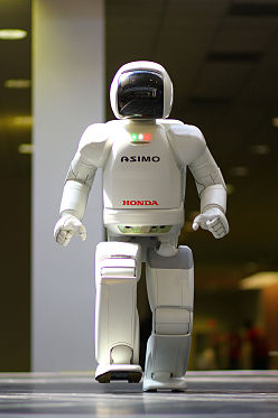
\includegraphics[width=0.2\textwidth]{figures/Introduccion/asimo.png}
		\caption{Robot Asimo}
		\label{fig.asimo}
		\end{center}
\end{figure}

El campo de la robótica es cada vez más popular y está en constante expansión. En la actualidad nos encontramos con múltiples ejemplos que integran la robótica en diferentes campos y tareas. Los robots comerciales e industriales son ampliamente utilizados y realizan tareas de forma más exacta o más barata que los humanos. Los robots, también, se emplean en trabajos demasiado sucios, peligrosos o tediosos para los humanos.\\

Hoy en día no solamente vemos robots industriales, como en cadenas de envasado de alimentos o cadenas de producción, sino que los robots cobran cada vez más importancia en los entornos domésticos. Las aspiradoras robóticas (Roomba, Dyson, Xiaomi…) han llegado a los hogares con éxito para facilitar una tarea doméstica necesaria. Los vehículos cada vez incorporan más tecnología robótica, como el aparcamiento automático en cualquier gama del mercado, asistentes de conducción autónoma (autopiloto de Tesla), o prototipos de coches autónomos que han lanzado grandes empresas como Google o Apple. Podemos ver robots en el campo de la medicina (como Da Vinci) que permiten operar siendo teleoperados desde cualquier parte del mundo; en el ámbito militar permitiendo desactivar bombas o realizar misiones rescate; en los almacenes de Amazon; o la creciente presencia de drones o robots aéreos.\\

Los robots tienen que interactuar con situaciones reales de forma robusta. Esto requiere que posean cierta inteligencia, la cual está presente en su software. Todas las aplicaciones actuales de robótica tienen cierta inteligencia, que reside en su software. Este software posee capas (drivers, \textit{middleware} y aplicaciones), y presenta unas características diferentes según su aplicación. En los últimos años, se han incorporado a los robots ordenadores personales, micros de bajo coste y sistemas operativos generalistas.

\begin{figure}[H]
  \begin{center}
    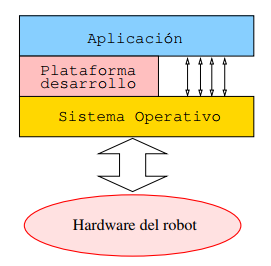
\includegraphics[width=0.4\textwidth]{figures/Introduccion/Esquema_Robot.png}
		\caption{Esquema del funcionamiento de un robot}
		\label{fig.Esquema_Robot}
		\end{center}
\end{figure}


\section{Software para robots}
Muchos robots poseen autonomía, la cual proviene del desarrollo de sistemas complejos, aplicaciones e infraestructuras que les dotan de inteligencia autónoma. El desarrollo de software robótico es similar al desarrollo de software en otros ámbitos, donde se parte de ciertos requisitos y se modela un diseño que será creado. Hace años el desarrollo de software robótico se realizaba adoptando soluciones ``ad hoc'', dotando a cada robot de un diseño específico, y con sensores y actuadores concretos. Esto suponía que no se podía aplicar el software desarrollado a otro robot, por lo que era necesario implementar de nuevo todo el software para un nuevo robot. En la actualidad, existen numerosas plataformas que permiten el desarrollo de aplicaciones robóticas de forma eficiente y genérica. Esto permite reutilizar gran parte de las aplicaciones creadas en otros robots, evitando el coste de realizar todo el proceso de nuevo.\\

Dotar al robot de cierta inteligencia conlleva desarrollar cierto software, el cual se suele programar apoyándose en herramientas, como los \textit{middleware} robóticos, los simuladores robóticos, o las  bibliotecas que facilitan algunos aspectos. A continuación, se exponen algunas de estas herramientas que se emplean en la actualidad.

\subsection{Middlewares robóticos}
En la actualidad existen numerosos \textit{middlewares} robóticos, que permiten gestionar la complejidad y heterogeneidad del hardware y las aplicaciones, promover la integración de nuevas tecnologías, simplificar el diseño de software, y ocultar la complejidad de los sensores. Algunos de los \textit{middlewares} robóticos más destacados son:

\begin{itemize}
\item \acrfull{ros} \footnote{\url{http://www.ros.org/}} ~\cite{middleware1}: Es una plataforma de software libre para el desarrollo de software de robots, que provee servicios estándar de un sistema operativo como la abstracción del hardware, el control de dispositivos de bajo nivel, mecanismos de intercambio de mensajes entre procesos y un conjunto de herramientas utilizadas ampliamente en robótica. La librería está orientada para un sistema UNIX, aunque se está adaptando a otros sistemas operativos como Fedora, Mac OS X, Arch, Gentoo, OpenSUSE, Slackware, Debian o Microsoft Windows, considerados como ``experimentales''.
\item Orca \footnote{\url{http://orca-robotics.sourceforge.net/}} ~\cite{middleware1}: Es una plataforma de software libre para el desarrollo de aplicaciones robóticas. Está orientada a componentes, los cuales se pueden ejecutar de manera independiente o conjunta para crear aplicaciones más complejas. Orca permite reutilizar código, de manera que se pueden emplear componentes robóticos ya creados.
\item Urbi ~\cite{urbi}: Es una plataforma de software multiplataforma de código abierto en C++ utilizada para desarrollar aplicaciones para robótica y sistemas complejos. Urbi es compatible con \acrshort{ros} y se puede emplear en los sistemas operativos Linux, Windows y MAC OS X.
\end{itemize}

\subsection{Simuladores robóticos}
El diseño de un robot es costoso y caro, lo que implica que muchos componentes necesarios para la construcción de los robots solamente estén disponibles para centros de investigación y corporaciones. Cuando se emplea un robot puede que el código desarrollado falle al probarlo, pudiendo incluso romperse algún robot.\\

Hoy en día existen numerosos simuladores robóticos, lo que permite a cualquier persona crear, programar y probar infinidad de robots de forma segura y económica. Algunos de los simuladores más empleados son:

\begin{itemize}
\item Gazebo \footnote{\url{http://gazebosim.org/}}: Es un simulador 3D de código abierto distribuido bajo licencia Apache 2.0. Este simulador se ha utilizado en ámbitos de investigación en robótica e Inteligencia Artificial. Es destacado por sus motores de físicas, motor de renderizado avanzado, soporte para \textit{plugins}, un amplio repertorio de robots comerciales, y una extensa gama de sensores y actuadores. Es fácil de integrar con \acrshort{ros}.
\item Stage \footnote{\url{http://playerstage.sourceforge.net/doc/stage-svn/}}: Simula robots móviles en el plano bidimensional y proporciona diversos tipos de sensores y actuadores. Su finalidad es ayudar a la investigación de sistemas autónomos de múltiples agente, para lo cual proporciona gran cantidad de dispositivos simultáneamente.
\item Orocos \footnote{\url{http://www.orocos.org/taxonomy/term/18}} ~\cite{orocos} ~\cite{orocos1}: Es un proyecto de software libre para el control de robots y máquinas. Soporta 4 bibliotecas C++: Real-Time Toolkit, Kinematics and Dynamics Library,  Bayesian Filtering Library, y  Orocos Component Library. Está orientado a componentes, permitiendo añadir funcionalidades de forma sencilla y sin recompilar todo el código.  Incluye paquetes complementarios tales como Filtros de Bayes, Librerías de control Dinámico y Cinemático o Visión. 
\item Webots \footnote{\url{https://www.cyberbotics.com/}} ~\cite{webots}: Es un simulador avanzado de robótica, que permite definir modelos propios, definir la física, escribir controladores para los robots y hacer simulaciones a gran velocidad. Se puede emplear en los sistemas operativos Linux, Windows y MacOS. Los lenguajes de programación que se pueden emplear son  C++, C y Java.
\end{itemize}

\subsection{Bibliotecas}
En el desarrollo del software robótico es conveniente emplear bibliotecas que ya resuelven funcionalidades como el reconocimiento de gestos, procesamiento de imágenes, o la estimación de posición. En la actualidad existen diferentes bibliotecas que se emplean en robótica, por ejemplo:

\begin{itemize}
\item OpenCV \footnote{\url{http://opencv.org/}}: Está dirigida a la visión por computador en tiempo real. Entre las áreas de aplicación de esta biblioteca destacan: segmentación y reconocimiento de objetos, reconocimiento de gestos, seguimiento del movimiento, estructura del movimiento,  y robots móviles.
\item PCL \footnote{\url{http://pointclouds.org/}} ~\cite{pcl} ~\cite{pcl1}:Es una biblioteca de código abierto para el procesamiento de imágenes 2D/3D. Incluye numerosos algoritmos para manejar nubes  de puntos en N dimensiones, y procesamiento tridimensional de las mismas. Se emplea en el manejo de información en sensores RGBD como Kinect.
\item AForge.NET ~\cite{AForge.NET}: Es un framework C\# de código abierto diseñado para desarrolladores e investigadores en los campos de Visión por Computadora e Inteligencia Artificial. Sus áreas de aplicación son: procesamiento de imágenes, redes neuronales, algoritmos genéticos, lógica difusa, aprendizaje de máquinas, robótica, etc.
\end{itemize}

\section{Docencia en robótica}
El propósito principal de este proyecto es la extensión de un entorno docente compuesto de varias prácticas para facilitar el aprendizaje de diferentes algoritmos de robótica. Estas prácticas utilizan técnicas robóticas próximas a las empleadas en la actualidad.\\

La robótica educativa es un medio de aprendizaje en el cual participan personas con motivación por el diseño y la construcción de creaciones propias. Esta disciplina se puede enseñar a estudiantes con muy diferentes niveles educativos. Ha crecido muy rápidamente en la última década y está en continuo desarrollo. Los robots están incorporándose en nuestra vida cotidiana, pasando de la industria a los hogares. El propósito de utilizar la robótica en la educación, a diferentes niveles de enseñanza, suele ir más allá de adquirir conocimiento en el campo de la robótica. Se pretende que el alumno sea capaz de aprender temas multidisciplinares (electrónica, informática, mecánica, física, etc), comprenda conceptos abstractos y complejos de ciencia y tecnología, y adquiriera competencias básicas que son necesarias en la sociedad de hoy día; como el aprendizaje colaborativo y la toma de decisión en equipo, entre otras.\\

La robótica genera entornos colaborativos donde los participantes pueden practicar las habilidades del siglo XXI, conocidas como las 4C:

\begin{itemize}
\item Creatividad: Implica generar nuevas ideas mejorando las que ya existen. Es necesario ponerse en diferentes puntos de vista en cada circunstancia, tener la mente abierta y ser receptivo ante nuevas ideas y conceptos. Ayuda a la resolución de problemas de manera más eficaz.
\item Pensamiento Crítico: Es imprescindible razonar con efectividad, claridad y precisión para desarrollar esta habilidad, reconociendo las conexiones que existen entre sistemas para resolver problemas y tomar decisiones. Se requiere practicar una correcta lógica de pensamientos para ver en cada situación los distintos puntos de vista.
\item Colaboración: Se basa en la capacidad para trabajar de forma eficaz y respetuosa en equipos diversos. Esta habilidad implica comprometerse con los demás en la consecución de un objetivo común. Es importante asumir la responsabilidad del trabajo colaborativo, así como las aportaciones de cada miembro del equipo.
\item Comunicación: Es la capacidad que permite intercambiar información de forma articulada, de dar y recibir retroalimentación de determinadas ideas con otras personas.
\end{itemize}

La robótica en la docencia intenta despertar el interés de los estudiantes transformando las asignaturas tradicionales en más atractivas e integradoras, ya que crea entornos de aprendizaje propicios que recrean los problemas del entorno que los rodea.\\

En el futuro, tener nociones básicas de esta disciplina será clave debido a que cada vez de forma más habitual se implantan robots en diferentes sectores laborales.

\subsection{Docencia en secundaria}

En los centros de enseñanza secundaria se imparte la robótica con frecuencia, ya que motiva a los alumnos. Esto permite a los alumnos adquirir conocimientos tecnológicos, así como aprender conceptos básicos de ciencias, tecnología, ingeniería y matemáticas. Es decir, se implanta el enfoque de educación \textit{\acrfull{stem}}. El concepto \acrshort{stem} se ha desarrollado con el fin de enseñar Ciencias y Tecnología de forma conjunta. Este método tiene dos características fundamentales:

\begin{itemize}
\item Enseñanza-aprendizaje de tecnología, ciencias, ingeniería y matemáticas de forma conjunta e integrada.
\item Se da un enfoque a la tecnología de aprender conocimientos para resolver problemas tecnológicos reales. 
\end{itemize}

La enseñanza de robótica en secundaria se realiza mediante plataformas físicas como los robots LEGO (Mindstorms, RCX, NXT, Evo, WeDo), placas Arduino, los kits de SolidWorks, etc. Se suelen enseñar conceptos básicos de sensores y actuadores empleando lenguajes gráficos como RCXcode, Scratch y mbot Blockly. \\

En los últimos años, diferentes universidades han planteado cursos orientados a promover el diseño de robots en estudiantes de secundaria. Un ejemplo es el departamento de  Electrónica de la Universidad de Alcalá, que creó el proyecto ``TuBot'' con el fin de que los alumnos puedan construir su propio robot e incluso participar en una competición con el mismo.\\

Es importante destacar el curso JdeRobot-Kids \footnote{\url{http://jderobot.org/JdeRobot-kids}}, que emplea mbot como robot móvil, una placa programable Arduino, y Python como lenguaje para introducir a los jóvenes los conceptos básicos, de tecnología, robótica y programación. De esta forma los alumnos podrán aprender de una forma más divertida conceptos interesantes de informática, electrónica y mecánica. El curso es fundamentalmente práctico, ya que la mejor manera de aprender es creando.

\subsection{Docencia en la universidad}
En la docencia universitaria se imparten clases de robótica en los Grados y los Postgrados, en concreto en escuelas de ingeniería. La enseñanza de robótica o materias similares como la inteligencia artificial, la visión por computador o el aprendizaje automático, se pueden impartir en el ámbito industrial, pero también en el ámbito informático.\\

En España, podemos ver la robótica integrada en el ``Grado en Ingeniería Robótica'' de la Universidad de Alicante, donde nos encontramos con asignaturas como ``Iniciación a la ingeniería robótica'', ``Mecanismos y modelado de robots'', ``Programación de robots'', o ``Control de robots''. La enseñanza de robótica la podemos encontrar en los Grados de ''Electrónica industrial y automática'' que encontramos en numerosas universidades. Cabe destacar la universidad Carlos III de Madrid, donde se pueden estudiar materias como ``Robótica Industrial'' o ``Robótica''. En diversas universidades se puede estudiar el Grado ``Ingeniería Electrónica, Robótica y Mecatrónica''. Las universidades de Málaga y Sevilla cuentan con esta titulación, en la cual se imparten asignaturas como ``Fundamentos de Robótica'', ``Laboratorio de Robótica'', ``Robótica y Automatización'', o ``Ampliación de Robótica''.\\

En los estudios de Postgrado se imparten más asignaturas de robótica, puesto que es una enseñanza más especializada. Existen Másteres destacados como el ``Máster de Visión Artificial'', el ``Máster Universitario en Ingeniería Mecatrónica'', o el ``Máster Universitario en Automática y Robótica'' en diferentes universidades. Estos estudios de Postgrado los podemos encontrar en universidades como la Universidad Rey Juan Carlos, la Universidad Carlos III de Madrid, la Universidad del País Vasco, o la Universidad Politécnica de Cataluña.\\

En el ámbito internacional, algunas asociaciones prestigiosas como ACM (Association for Computing and Machinery) y la IEEE-CS (IEEE Computer Society) ven la robótica como un área de conocimiento imprescindible en estudios de ingeniería, informática y sistemas inteligentes. Se pueden destacar universidades especializadas en robótica como el MIT, Stanford, Georgia Institute of Technology, etc.\\

La asignatura de robótica habitualmente se imparte de forma práctica facilitando el aprendizaje de contenidos teóricos al alumno. Es común el uso de plataformas para la programación de robots. Algunas de las plataformas más destacadas son \acrshort{ros} \footnote{\url{http://www.ros.org/}}, o MATLAB con el paquete Simulink \footnote{\url{https://es.mathworks.com/products/simulink.html}}.\\

Cabe destacar The ConstructSim, que es útil para realizar simulaciones en la web. Esta plataforma web en la nube permite emplear una gran lista de simuladores por medio de un navegador web. De esta forma los usuarios no tienen que instalar nada, ni siquiera en sus navegadores.

\section{Entorno Docente JdeRobot-Academy}
La Universidad Rey Juan Carlos cuenta con el \textit{middleware} robótico JdeRobot, que tiene asociado un entorno académico conocido como JdeRobot-Academy. Este entorno educativo se ha empleado con éxito en diferentes asignaturas, como ``Visión en Robótica'' del Máster de Visión Artificial, o ``Robótica'' del Grado de Ingeniería Telemática. Asimismo, la Universidad ofrece cursos de introducción a la robótica y los drones, empleando dicha plataforma.\\

Los ejes principales de JdeRobot-Academy son: (a) lenguaje Python (por su sencillez y potencia), (b) simulador Gazebo (permite aprender robótica aunque no se disponga de robots reales, y permite tener un repertorio de robots variados ---drones, formula1, brazos, aspiradoras, etc.--- con los que enfocar aspectos muy variados de la robótica) y (c) foco en el algoritmo en vez de en el \textit{middleware} ocultando los detalles de la infraestructura.\\


El entorno cuenta con un conjunto de prácticas. En cada una se plantea un problema robótico que tiene que resolver el alumno. En cada práctica se pueden distinguir varias capas, que influyen en el desarrollo del diseño de las prácticas. La capa de nivel más bajo, que será la primera que se crea, es la creación de la infraestructura de la práctica, lo que supone la creación de los modelos necesarios, los \textit{plugins} que emplearán estos modelos, y el entorno simulado donde navegará el robot. \\

Por cada una de las prácticas se incluye un componente académico que le permitirá al alumno realizar la solución de las prácticas. Cada uno de estos componentes proporciona una interfaz gráfica (\acrshort{gui}) específica para esa práctica y código auxiliar de ayuda a la resolución de las prácticas. También suele incluir un evaluador automático, que permite llevar a cabo la corrección de las prácticas. En las prácticas se harán las conexiones necesarias del software del alumno con los sensores y actuadores que se empleen. El propósito de los componentes académicos es permitir la abstracción por parte de los alumnos de los elementos complejos que no son parte de la resolución de las prácticas. De esta forma, el alumno lo único que tendrá que hacer es programar la solución de cada algoritmo que se le propone.
\begin{figure}[H]
  \begin{center}
    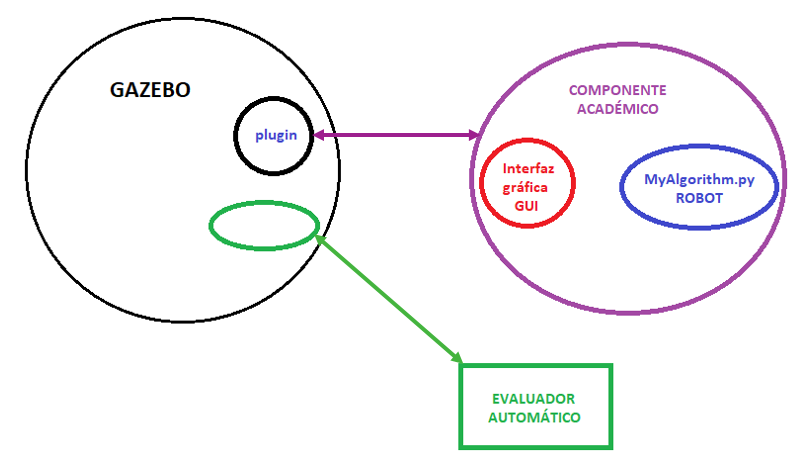
\includegraphics[width=0.6\textwidth]{figures/Introduccion/estructura.png}
		\caption{Estructura}
		\label{fig.estructura}
		\end{center}
\end{figure}

Se han creado los componentes académicos siguiendo una arquitectura software que permite facilitar el desarrollo de las prácticas a los alumnos, los cuales únicamente deberán realizar la solución, ya sea el pilotaje en función de los datos que proporcionan los sensores  o la realización de la planificación y el pilotaje. Los componentes cargan el código escrito por el alumno en el fichero MyAlgorithm.py (donde se lleva a cabo la resolución), mostrando en la interfaz las pruebas o soluciones que realicen los alumnos. En la Figura~\ref{fig.estructura} podemos ver la estructura que tiene cada una de las prácticas.\\

Las prácticas se pueden realizar sobre robots simulados o reales, aunque lo más habitual es emplear robots simulados. Se apoyan en el simulador Gazebo, y se usa como lenguaje de programación Python. El principal sistema operativo para emplear esta plataforma es Linux. Sin embargo, se ha utilizado la interfaz web Gazebo para poder lanzarlo en Windows y MacOS mediante el empleo de Dockers.\\

A continuación, se presentan algunas de las prácticas ya desarrolladas en el entorno docente JdeRobot-Academy:

\begin{itemize}
\item Fórmula 1 \footnote{\url{https://www.youtube.com/watch?v=eNuSQN9egpA}}: sigue líneas. En esta práctica el alumno debe programar el comportamiento de un coche Fórmula 1 para que realice un control PID siguiendo la línea roja pintada en el circuito de carreras. Para ello el robot posee sensores de posición y una cámara. La interfaz de movimiento es simple puesto que admite órdenes de velocidad lineal o velocidad de giro.
\begin{figure}[H]
  \begin{center}
    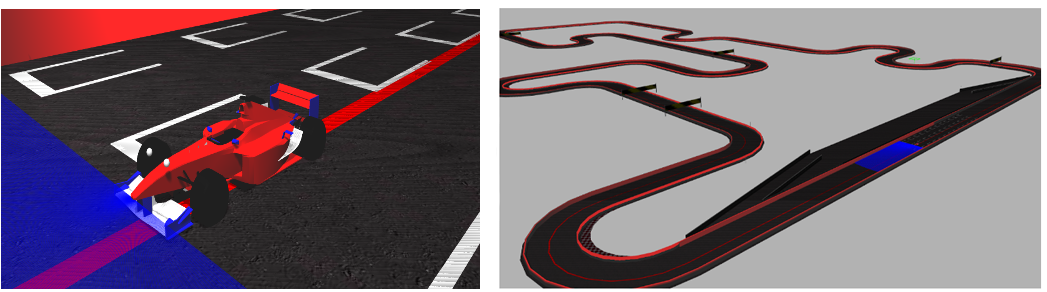
\includegraphics[width=0.8\textwidth]{figures/Introduccion/F1.png}
		\caption{Fórmula 1 y circuito de Gazebo}
		\label{fig.F1}
		\end{center}
\end{figure}
\item Visión \footnote{\url{http://jderobot.org/store/jmplaza/uploads/teaching/teachingrobotics-reconstruccion3D.mp4}}: reconstrucción 3D. En esta práctica el alumno debe lograr que un robot Pioneer reproduzca en 3D los elementos que están en frente del mismo. El robot cuenta con un par de cámaras estéreo. Para abordar el problema adecuadamente el alumno deberá programar un algoritmo de reconstrucción 3D clásico: detección de puntos de interés en el par de imágenes, emparejamiento de pixeles homólogos entre ambas, y triangulación espacial para calcular el punto tridimensional que origina cada pareja de pixeles homólogos. Esta práctica aborda técnicas de procesado de imagen y percepción visual.
\begin{figure}[H]
  \begin{center}
    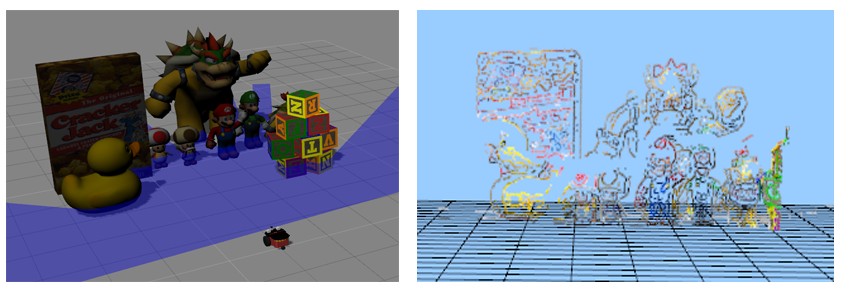
\includegraphics[width=0.8\textwidth]{figures/Introduccion/3D.png}
		\caption{Pioneer en el mundo de Gazebo y reconstrucción 3D}
		\label{fig.3D}
		\end{center}
\end{figure}
\item Control visual en drones \footnote{\url{https://www.youtube.com/watch?time_continue=96&v=BoDchf_6yMQ}}: sigue a la tortuga. En esta práctica el alumno debe conseguir que un drone siga a un robot Turtlebot que se desplaza por el suelo. Para lograr este objetivo el alumno deberá realizar los filtros de percepción visual necesarios para que el drone identifique al Turtlebot, así como programar el movimiento del drone para que siga al robot de forma adecuada. Esta práctica permite enseñar técnicas de percepción visual, de control reactivo, control basado en casos y de controladores PID.
\begin{figure}[H]
  \begin{center}
    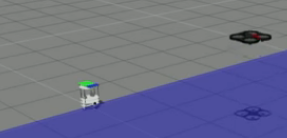
\includegraphics[width=0.5\textwidth]{figures/Introduccion/Tortuga.png}
		\caption{Drone en el mundo de Gazebo}
		\label{fig.Tortuga}
		\end{center}
\end{figure}
\end{itemize}

El objetivo general de este proyecto es ampliar las posibilidades de esta plataforma docente, creando nuevas prácticas y mejorando alguna ya existente. En los próximos capítulos abordaremos todos los elementos necesarios para conseguir este objetivo. En el capítulo ~\ref{cap.objetivos} cubriremos los objetivos que se han marcado en el proyecto, así como los requisitos para cumplirlos y la metodología empleada. En el capítulo ~\ref{cap.infraestructura} se expondrán la infraestructura utilizada durante el trabajo. En los capítulos ~\ref{cap.gpp}, ~\ref{cap.roomba} y ~\ref{cap.autoparking}, se abordarán las prácticas que se han mejorado o creado. Por último, en el séptimo capítulo se expondrán las conclusiones obtenidas al realizar el proyecto, así como las posibles líneas futuras a seguir.